\documentclass[12pt]{article}

\usepackage{amsmath}
\usepackage[dvips]{graphicx}
\usepackage{psfrag}
\usepackage{fancyhdr}
\usepackage{lastpage}
% \usepackage{natbib}
\usepackage[usenames,dvipsnames]{color}
\usepackage[
  colorlinks=true,
  urlcolor=blue
  ]{hyperref}
%\usepackage{listings}
\usepackage{xspace}
\usepackage{upquote}
\usepackage[T1]{fontenc}
\usepackage{textcomp}

%\lstset{
%    literate={~} {$\sim$}{1}
%}


\topmargin       -0.5truein
\headsep          0.5truein
\headheight       0.0truein
\oddsidemargin   -0.4truein
\evensidemargin  -0.4truein
\textwidth        6.5truein
\textheight       9.0truein

\addtolength{\hoffset}{1.0cm}
\newcommand{\mytilde}{\raise.17ex\hbox{$\scriptstyle\mathtt{\sim}$}}
\pagestyle{fancyplain}
\lhead{}
%\chead{\small DFT exercises for Quantum Mobile 2021}
\rhead{}
\cfoot{Page~\thepage~of~\pageref{LastPage}}

% \newcommand{\code}[1]{{\centering \textsc{#1} \\}}
\newcommand{\code}[1]{
\begin{quotation}
  #1 
\end{quotation}
}

\def\QE{\textsc{Quantum ESPRESSO}\xspace}

\def\red#1{\textcolor{red}{#1}}

\begin{document}

\title{{\bf Instructions on setting up Quantum Mobile}}

%\author{Iurii Timrov\\
%    {\it THEOS and NCCR-MARVEL, \'Ecole Polytechnique F\'ed\'erale de Lausanne}}
%\date
  
\maketitle
%\tableofcontents
%\newpage


\noindent
Computer programs are not always so easy to install and maintain. 
One of the easiest ways to deal with this issue in the context of learning the use
of a new tool, so that the person learning does not need to first start troubleshooting
configuration problems before actually testing the tool itself, is to provide
the necessary codes pre-installed inside of a self-contained working environment
called "Virtual Machine".
These virtual machines can be run using different programs and effectively work
as a "machine inside the machine", with its own libraries, programs and files
and with limited points of contact with the "external device" that is being used
to run it (your physical computer).

\vskip 0.5cm

\noindent
To set this up, you will first need to download and install
\href{https://www.virtualbox.org/}{VirtualBox}
version 6.1.22 or later: this is the program that we will use to run the virtual
machine. Then you also need to download the virtual machine itself (4.82 Gb),
\href{https://github.com/marvel-nccr/quantum-mobile/releases/tag/20.03.1}
{Quantum Mobile version 21.06.04},
and import it into Virtualbox (note, this will occupy about 13 Gb of disk space) by going to the "File" menu and choosing "Import Appliance".
See Fig.~\ref{import_vm} for an idea on how VirtualBox looks like and where
to find the "Import Appliance" option; you can also consult the
\href{https://github.com/marvel-nccr/quantum-mobile/wiki/Frequently-Asked-Questions}
{FAQ of Quantum Mobile}
for further information or troubleshooting.

\begin{figure}[h!]
\centering
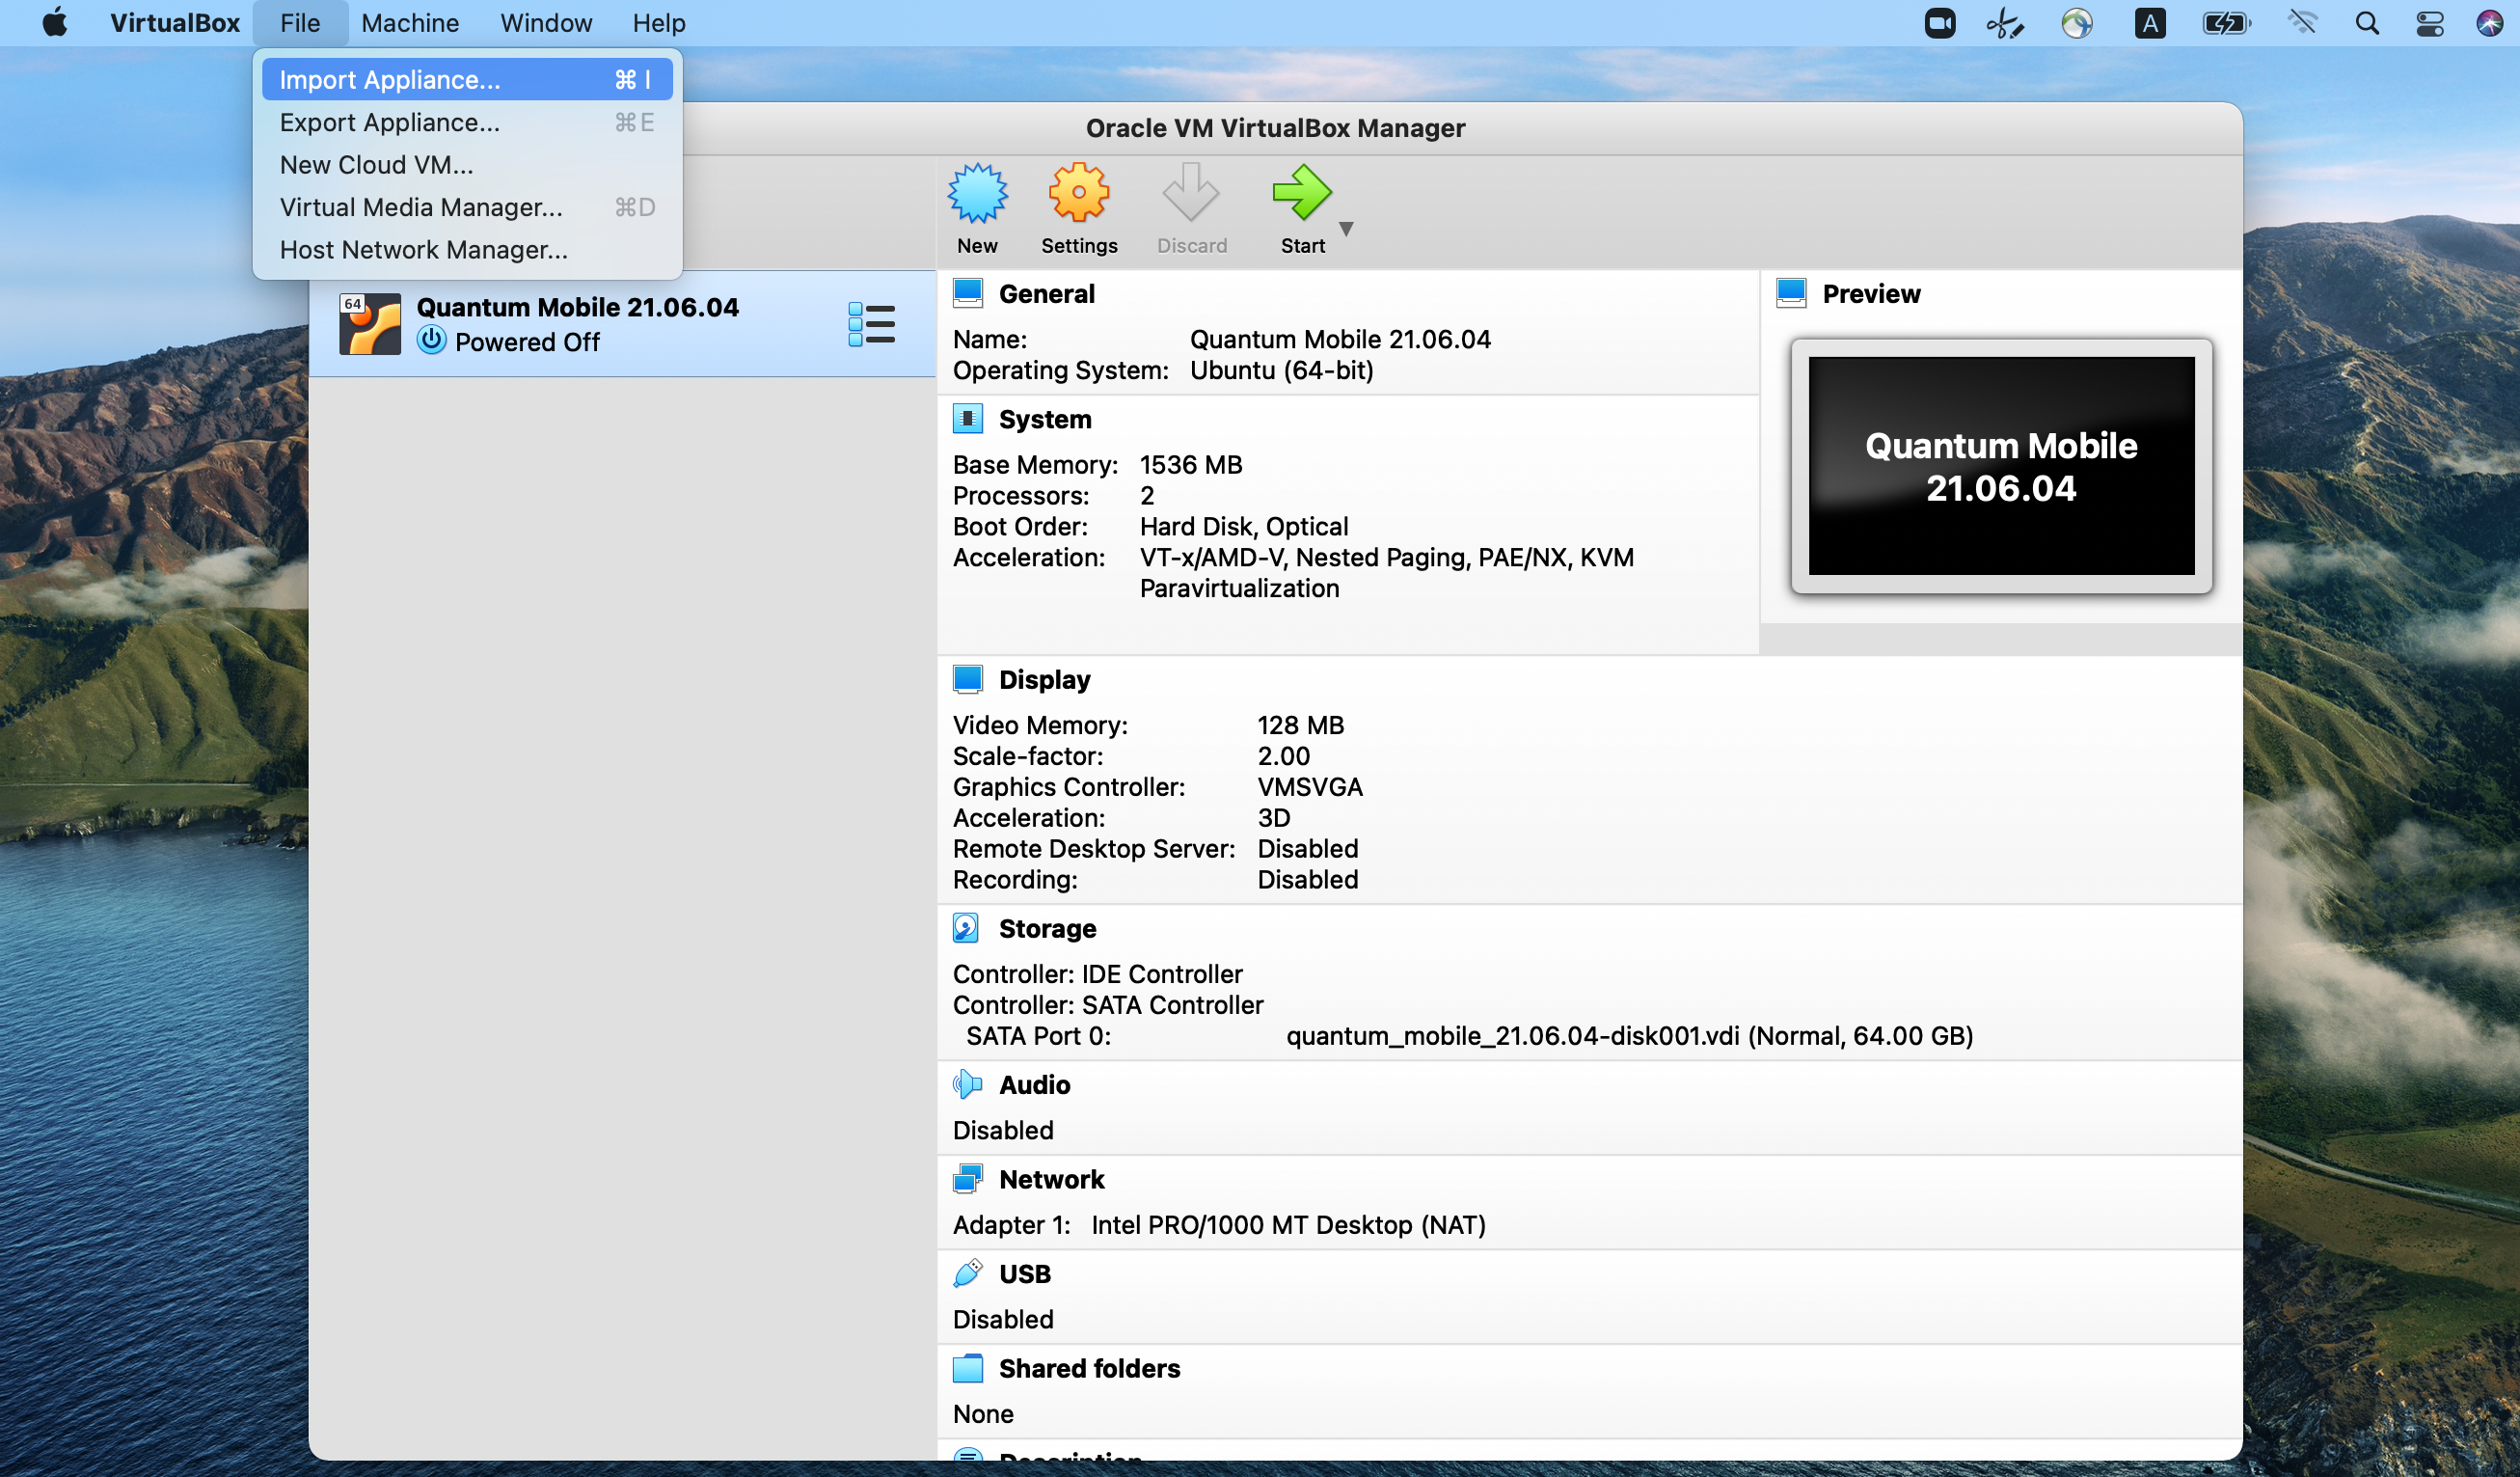
\includegraphics[height=270pt]{import.png}
\caption{VirtualBox interface and "import" option (in MacOS)}
\label{import_vm}
\end{figure}

\vskip 0.5cm

\noindent
Next, press the "Start" button (green right arrow) to run Quantum Mobile (see Fig.~\ref{import_vm}). You should see what is shown in Fig.~\ref{QM}. If there are some problems, try to find a solution in the \href{https://quantum-mobile.readthedocs.io/en/latest/users/troubleshoot.html}{Troubleshooting page}.\\

\noindent
Finally, you need to download the material for this tutorial. To do so, in the Quantum Mobile window open a Chromium Web Browser, go to the webpage 
\href{https://github.com/materialscloud-org/learn-fireside-hubbard}
{https://github.com/materialscloud-org/learn-fireside-hubbard},
click on the green button "Code", and then click on "Download ZIP".
Next, close the browser and go to the "Files" folder on the left-hand side of the desktop in Quantum Mobile, next go to "Downloads", and then double-click on the downloaded file "learn-fireside-hubbard-main.zip" and press "Extract" in the upper left corner of the window. Lastly, go to the extracted folder "learn-fireside-hubbard-main". Now you are ready to get started with the tutorial. Note that in the following we will work in the terminal, so you should be familir with \href{http://mally.stanford.edu/~sr/computing/basic-unix.html}{basic Unix commands}.

\begin{figure}[h!]
\centering
\includegraphics[height=285pt]{QuantumMobile.png}
\caption{Quantum Mobile window.}
\label{QM}
\end{figure}


\end{document}
